\documentclass[10pt]{article}
\usepackage[letterpaper,margin=0.68in,headheight=15pt,footskip=28pt]{geometry}
\usepackage[T1]{fontenc}
\usepackage{lmodern}
\usepackage{microtype}
\usepackage{amsmath,amssymb,bm,mathtools}
\usepackage{graphicx}
\usepackage{booktabs,tabularx,array,longtable}
\usepackage{enumitem}
\usepackage{xcolor}
\usepackage{hyperref}
\usepackage{fancyhdr}
\usepackage{lastpage}
\usepackage{caption}
\usepackage{float}
\usepackage{parskip}
\usepackage{titlesec}

\definecolor{posmblue}{RGB}{27,102,142}
\definecolor{lightblue}{RGB}{239,246,249}
\definecolor{warnbg}{RGB}{252,247,235}
\definecolor{grayline}{RGB}{135,145,152}
\hypersetup{colorlinks=true,linkcolor=black,urlcolor=posmblue,citecolor=posmblue,pdfauthor={Photonics and Optical Sciences Club at Minnesota},pdftitle={Synthetic Intermodulation Transfer Spectroscopy Theory Packet}}
\setlist{leftmargin=1.45em,itemsep=2pt,topsep=3pt}
\titleformat{\section}{\Large\bfseries}{\thesection}{0.65em}{}
\titleformat{\subsection}{\large\bfseries}{\thesubsection}{0.6em}{}
\titleformat{\subsubsection}{\normalsize\bfseries}{\thesubsubsection}{0.55em}{}
\pagestyle{fancy}
\fancyhf{}
\fancyhead[L]{\small POSM - Synthetic Intermodulation Transfer Spectroscopy}
\fancyhead[R]{\small Theory / Research Brief}
\renewcommand{\headrulewidth}{0.35pt}
\fancyfoot[L]{\scriptsize $\bullet\ \bullet\ \bullet\ \bullet\ \bullet$}
\fancyfoot[R]{\scriptsize \thepage\ of \pageref{LastPage}}

\newcommand{\note}[1]{\begin{center}\fcolorbox{posmblue}{lightblue}{\begin{minipage}{0.93\linewidth}\textbf{POSM note.} #1\end{minipage}}\end{center}}
\newcommand{\warningbox}[1]{\begin{center}\fcolorbox{grayline}{warnbg}{\begin{minipage}{0.93\linewidth}\textbf{Important.} #1\end{minipage}}\end{center}}
\newcommand{\vect}[1]{\bm{#1}}
\newcommand{\dd}{\mathrm{d}}
\newcommand{\ii}{\mathrm{i}}

\begin{document}

% COVER
\thispagestyle{fancy}
\vspace*{0.3in}
\begin{center}
{\small POSM Research Packet \hfill Nonlinear Spectroscopy $\bullet$ Laser Locking $\bullet$ FPGA Readout}\par
\vspace{0.35in}
\colorbox{black}{\parbox{0.76\linewidth}{\centering\vspace{0.27in}{\color{white}\fontsize{46}{50}\selectfont\bfseries POSM}\vspace{0.27in}}}
\vspace{0.48in}

{\fontsize{24}{29}\selectfont\bfseries Synthetic Intermodulation Transfer Spectroscopy}\\[0.12in]
{\Large Theory Packet for Engineered Atomic Frequency Discrimination}\\[0.26in]
\rule{1.35in}{0.45pt}\\[0.28in]
{\large Photonics and Optical Sciences Club at Minnesota (POSM)}\\[0.08in]
{\normalsize Research draft - August 10, 2026}
\end{center}

\vspace{0.42in}
\note{\textbf{Project mission.} Test whether two coherent MTS modulation tones expose useful atomically resonant combination-frequency channels and whether the full set of fundamental and intermodulation (IM) quadratures can be coherently combined into a synthetic frequency discriminator that outperforms every individual conventional MTS channel on a declared metric.}

\textbf{Core research claim to earn, not assume.} Two-tone MTS may create a multichannel nonlinear RF measurement of detuning. If the channels carry complementary frequency information, the noise-optimal synthetic combination can lower equivalent frequency noise; if their line shapes differ, constrained combinations may also enlarge the monotonic capture region or suppress selected systematics.

\textbf{Current novelty boundary.} Two-tone FM spectroscopy, multi-frequency MTS, velocity-comb MTS, and a 2026 dual-frequency MTS patent already exist. The proposed research is narrower: true output channels at $p\Omega_1+q\Omega_2$ plus joint complex/covariance-aware synthesis. No ``first'' claim is justified until a dedicated literature and patent search is completed.

\textbf{How to read this packet.} Sections 1--4 build the optical and RF theory. Sections 5--7 derive the synthetic discriminator and engineered objectives. Sections 8--10 connect the theory to POSM hardware and define decisive experiments. Sections 11--13 map novelty, failure modes, and a paper-ready program.

\newpage
\tableofcontents
\newpage

\section{Research Question and System Boundary}

\subsection{The one-sentence version}
Conventional MTS asks one RF component of a nonlinear atom-light interaction to serve as the laser-frequency sensor. Synthetic intermodulation transfer spectroscopy (S-IMTS) asks whether a two-tone pump creates a \emph{family} of useful complex RF observables and whether those observables can be combined optimally to create a better frequency discriminator.

The proposal should be judged in three progressively stronger stages:
\begin{enumerate}
\item \textbf{Existence:} atomically resonant combination-frequency channels $Z_{p,q}(\Delta)$ are measurable above non-atomic IM backgrounds.
\item \textbf{Complementarity:} at least some IM channels contain frequency information that is not redundant with the conventional fundamental channel.
\item \textbf{Utility:} a predeclared synthetic discriminator improves a meaningful quantity under equal resource constraints: equivalent frequency noise, systematic sensitivity, monotonic capture range, or closed-loop performance.
\end{enumerate}

\subsection{Why POSM is unusually well positioned}
The existing POSM FPGA lock packet deliberately separates a latency-critical analog-demodulated MTS channel from a simultaneously digitized raw RF monitor. The baseline uses ADC\_CH0 for the analog-demodulated error, ADC\_CH1 for the raw photodiode RF branch, an AD9959 for coherent RF generation, a fast current actuator, and a deliberately short FPGA path targeting at least 1 MHz closed-loop bandwidth. This means S-IMTS can begin as an \emph{observer experiment} on the raw channel without breaking the known fast lock architecture.

A low-risk architecture is therefore:
\begin{verbatim}
legacy analog MTS -> ADC_CH0 -> short FPGA PI -> fast current actuator
                              (baseline / safety lock)

AD9959 tone f1 --\
                  > RF combiner -> EOM -> Rb MTS -> raw RF -> ADC_CH1
AD9959 tone f2 --/                                |
                                                 +-> digital demod bank
                                                     Z_10, Z_01,
                                                     Z_1-1, Z_11,
                                                     Z_2-1, Z_-12, ...
\end{verbatim}

Only after the IM channel map is understood should a synthetic error replace or supplement the baseline error signal.

\section{Conventional Single-Tone MTS: Minimum Theory Needed}

\subsection{Phase-modulated pump field}
For a carrier at optical angular frequency $\omega_0$ with phase modulation index $\beta$ and RF modulation frequency $\Omega$,
\begin{equation}
E_p(t)=E_0 e^{\ii\omega_0 t}e^{\ii\beta\cos(\Omega t+\phi)}.
\end{equation}
The Jacobi--Anger expansion gives
\begin{equation}
e^{\ii\beta\cos\theta}=\sum_{m=-\infty}^{\infty}\ii^mJ_m(\beta)e^{\ii m\theta},
\end{equation}
so the pump contains an optical sideband ladder
\begin{equation}
E_p(t)=E_0\sum_m a_m e^{\ii(\omega_0+m\Omega)t},\qquad
a_m=\ii^mJ_m(\beta)e^{\ii m\phi}.
\end{equation}
The total optical power is redistributed among these lines while remaining constant in the ideal lossless phase modulator:
\begin{equation}
\sum_{m=-\infty}^{\infty}|J_m(\beta)|^2=1.
\end{equation}

\subsection{How modulation reaches the probe}
In the standard coherent picture, the strong modulated pump and an initially unmodulated counterpropagating probe interact through the resonant atomic nonlinearity. A third-order polarization term has the schematic form
\begin{equation}
P^{(3)}(\omega_a+\omega_b-\omega_c)
=\epsilon_0\chi^{(3)}(\omega_a,\omega_b,-\omega_c)E_aE_bE_c^*.
\end{equation}
Pump components separated by $\Omega$ can therefore generate probe sidebands separated from the probe carrier by $\Omega$. In an isolated cycling transition this four-wave-mixing picture is especially useful and explains the characteristic background-free MTS response. However, detailed density-matrix studies show that neighboring transitions, polarization, optical pumping, and even spontaneous-emission-mediated contributions can matter on other transitions. The present proposal therefore uses the $\chi^{(3)}$ picture as a perturbative organizing model, not as a universal claim that every MTS signal is exclusively coherent FWM.

\subsection{Photodetection and demodulation}
Write the probe after the atomic medium as
\begin{equation}
E_s(t)=B_0 e^{\ii\omega_s t}+B_+e^{\ii(\omega_s+\Omega)t}+B_-e^{\ii(\omega_s-\Omega)t}+\cdots .
\end{equation}
The photodiode measures $i(t)\propto |E_s(t)|^2$. The complex coefficient near $\Omega$ is approximately
\begin{equation}
Z_1\propto B_+B_0^*+B_0B_-^*+\cdots .
\end{equation}
A coherent reference extracts an arbitrary quadrature
\begin{equation}
e_\theta(\Delta)=\Re\{Z_1(\Delta)e^{-\ii\theta}\}.
\end{equation}
Conventional MTS chooses one $\theta$ and one RF frequency, then uses the zero-crossing slope
\begin{equation}
D=\left.\frac{\partial e_\theta}{\partial\nu}\right|_{\nu_0}
\end{equation}
as the local frequency discriminant. Existing optimization literature tunes modulation frequency, modulation index, beam sizes, powers, and phase to improve amplitude, slope, noise, or robustness.

\warningbox{For S-IMTS, ``larger slope'' is not by itself the correct performance objective. The quantity that matters for local frequency sensing is slope relative to the full noise covariance, and for a real lock the discriminator must also have acceptable dynamic phase, systematic sensitivity, and capture behavior.}

\section{Two-Tone Phase Modulation and the 2D Optical Sideband Lattice}

\subsection{Exact two-tone expansion}
Let the pump phase be
\begin{equation}
\Phi(t)=\beta_1\cos(\Omega_1t+\phi_1)+\beta_2\cos(\Omega_2t+\phi_2).
\end{equation}
Because the exponentials factor,
\begin{align}
E_p(t)&=E_0e^{\ii\omega_0t}e^{\ii\beta_1\cos(\Omega_1t+\phi_1)}e^{\ii\beta_2\cos(\Omega_2t+\phi_2)}\\
&=E_0\sum_{m,n}a_{m,n}e^{\ii(\omega_0+m\Omega_1+n\Omega_2)t},
\end{align}
with
\begin{equation}
a_{m,n}=\ii^{m+n}J_m(\beta_1)J_n(\beta_2)e^{\ii(m\phi_1+n\phi_2)}.
\end{equation}
Thus the optical field is naturally indexed by the integer lattice $(m,n)$ rather than a one-dimensional sideband order.

\begin{figure}[H]
\centering
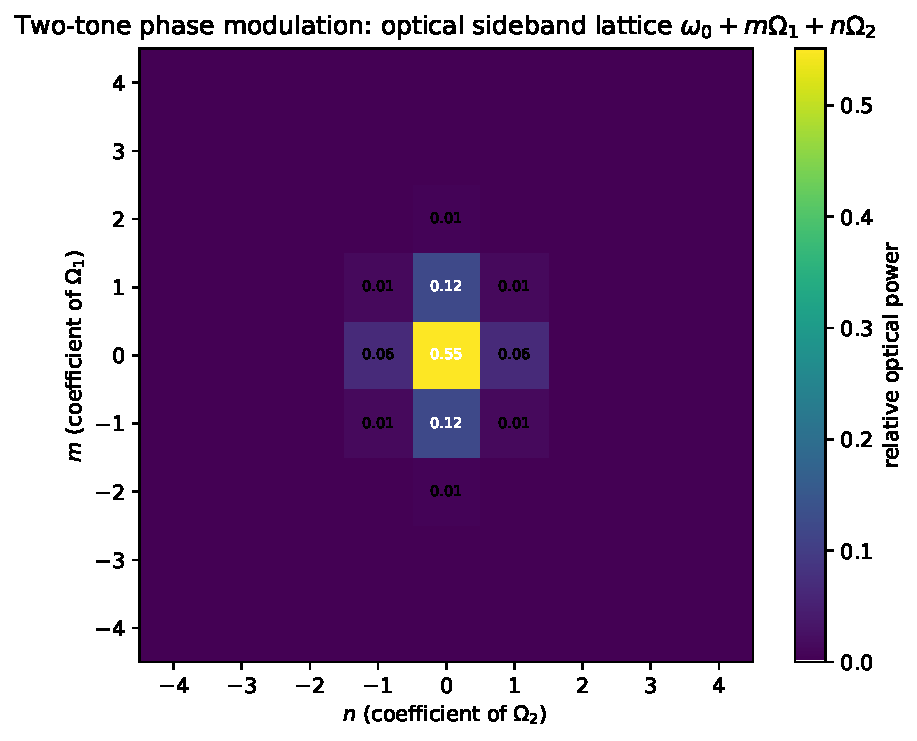
\includegraphics[width=0.69\linewidth]{../figures/fig1_sideband_lattice.pdf}
\caption{Illustrative two-tone optical sideband lattice for $\beta_1=0.85$ and $\beta_2=0.65$. Values shown are relative optical powers $|J_m(\beta_1)J_n(\beta_2)|^2$. This is an ideal EOM field calculation, not an atomic MTS prediction.}
\end{figure}

\subsection{Small-index scaling}
For small $\beta$,
\begin{equation}
J_k(\beta)\sim\frac{1}{|k|!}\left(\frac{\beta}{2}\right)^{|k|}
\end{equation}
(up to sign for negative order). Therefore a field component $(m,n)$ approximately scales as
\begin{equation}
|a_{m,n}|\propto \beta_1^{|m|}\beta_2^{|n|}.
\end{equation}
This gives a first diagnostic for modulation-order scaling, but it is not yet the scaling of the detected atomic IM signal because that signal includes atomic susceptibilities and multiple interfering paths.

\subsection{Important conceptual caution}
An ideal phase modulator driven by two tones already creates optical field components at combination offsets $m\Omega_1+n\Omega_2$. Therefore observing electrical power at a combination frequency is \emph{not, by itself}, proof that the rubidium generated an intermodulation product. Pure phase modulation has constant optical intensity in the ideal limit, but any downstream dispersion, absorption, EOM imperfection, RF amplifier nonlinearity, photodiode nonlinearity, or atomic response can convert the structured phase spectrum into intensity beats. Atomic attribution requires controlled subtraction and scaling tests described later.

\section{Atomic Generation and Transfer of Combination-Frequency Channels}

\subsection{Difference-index selection rule}
Consider pump lattice components
\begin{equation}
\omega_{m,n}=\omega_0+m\Omega_1+n\Omega_2
\end{equation}
and
\begin{equation}
\omega_{m',n'}=\omega_0+m'\Omega_1+n'\Omega_2.
\end{equation}
A third-order process involving these pump components and the probe can generate a probe component at
\begin{align}
\omega_{\text{new}}
&=\omega_s+\omega_{m,n}-\omega_{m',n'}\\
&=\omega_s+p\Omega_1+q\Omega_2,
\end{align}
where
\begin{equation}
p=m-m',\qquad q=n-n'.
\end{equation}
This gives the central S-IMTS channel labeling
\begin{equation}
\boxed{\Omega_{p,q}=p\Omega_1+q\Omega_2.}
\end{equation}
Low-order channels include $(1,0)$ and $(0,1)$ fundamentals, $(1,-1)$ difference, $(1,1)$ sum, and IM3-style $(2,-1)$ and $(-1,2)$ products.

\subsection{Perturbative generated-sideband model}
A useful schematic amplitude is
\begin{equation}
\boxed{
B_{p,q}(\Delta)\propto
\sum_{m,n}
\chi^{(3)}_{m,n;p,q}(\Delta)
\,a_{m,n}a_{m-p,n-q}^*\,E_s .}
\end{equation}
The object $\chi^{(3)}_{m,n;p,q}$ is deliberately broad: it may depend on detuning, velocity class, hyperfine and Zeeman structure, polarization, power broadening, optical pumping and relaxation. Multiple lattice pairs can contribute to the same $(p,q)$ output and therefore interfere coherently.

For counterpropagating pump/probe MTS, the wave-vector difference between two co-propagating pump sidebands is small compared with optical wave vectors, so the generated sideband can satisfy an approximately probe-directed phase-matching relation. The exact multilevel model should use the complete atomic Hamiltonian rather than a scalar $\chi^{(3)}$.

\subsection{Doppler average}
For velocity $v$ along the beam, each optical detuning shifts by $kv$. A microscopic channel amplitude is therefore velocity-dependent:
\begin{equation}
B_{p,q}(\Delta)=\int_{-\infty}^{\infty}B_{p,q}(\Delta,v)f_{\rm MB}(v)\,\dd v.
\end{equation}
The familiar MTS sub-Doppler selection emerges from the counterpropagating pump/probe resonance conditions. With two tone spacings, different lattice pairs can address different combinations of velocity and hyperfine pathways, which is one reason the IM line shapes need not be scalar copies of the conventional signal.

\subsection{Full two-frequency density-matrix / Floquet route}
A future first-principles model can start from
\begin{equation}
\dot\rho=-\frac{\ii}{\hbar}[H_0+V(t),\rho]+\mathcal L(\rho),
\end{equation}
where $V(t)$ contains the probe plus two-tone pump. Because the Hamiltonian is quasiperiodic at $\Omega_1$ and $\Omega_2$, expand
\begin{equation}
\boxed{\rho(t)=\sum_{p,q}\rho_{p,q}e^{\ii(p\Omega_1+q\Omega_2)t}.}
\end{equation}
Substitution yields a two-dimensional set of coupled algebraic/Floquet equations for the Fourier components $\rho_{p,q}$. The optical polarization channel follows from
\begin{equation}
P_{p,q}=N\,\mathrm{Tr}(\vect d\rho_{p,q}),
\end{equation}
then requires velocity averaging and Maxwell propagation.

\note{The full Floquet-density-matrix calculation is not required before the first experiment. A strong first paper can be empirical/perturbative: prove atomic IM channels, map their complex line shapes and scaling, and demonstrate a synthetic discriminator. The microscopic model becomes necessary only if the paper claims a specific atomic pathway or predicts an optimal channel from first principles.}

\section{From Generated Optical Sidebands to Measured RF Channels}

\subsection{General photodetector coefficient}
Write the transmitted probe field as
\begin{equation}
E_s(t)=\sum_{p,q}B_{p,q}e^{\ii(\omega_s+p\Omega_1+q\Omega_2)t}.
\end{equation}
The photodiode current is proportional to
\begin{equation}
|E_s|^2=\sum_{p,q}\sum_{r,s}B_{p,q}B_{r,s}^*e^{\ii[(p-r)\Omega_1+(q-s)\Omega_2]t}.
\end{equation}
Thus the complex RF coefficient at channel $(u,v)$ is
\begin{equation}
\boxed{Z_{u,v}\propto\sum_{r,s}B_{r+u,s+v}B_{r,s}^*.}
\end{equation}
If the probe carrier dominates, a weak-sideband approximation gives
\begin{equation}
Z_{u,v}\approx B_{u,v}B_{0,0}^*+B_{0,0}B_{-u,-v}^*.
\end{equation}
This is the direct multitone analogue of carrier--sideband beating in conventional FM/MTS detection.

\subsection{Complex demodulation}
For every chosen electrical frequency $\Omega_{p,q}$, digital synchronous detection returns
\begin{equation}
Z_{p,q}(\Delta)=I_{p,q}(\Delta)+\ii Q_{p,q}(\Delta).
\end{equation}
A scalar error signal for that channel is
\begin{equation}
e_{p,q,\theta}(\Delta)=\Re\{Z_{p,q}(\Delta)e^{-\ii\theta}\}.
\end{equation}
The natural coherent reference phase includes the input phases approximately as
\begin{equation}
\theta_{p,q}\sim p\phi_1+q\phi_2+\theta_{\rm chain},
\end{equation}
where $\theta_{\rm chain}$ contains atomic and electronic phase. For a time-invariant nondegenerate nonlinear process, varying $\phi_1$ or $\phi_2$ often rotates the IM phasor predictably; it does not necessarily change its magnitude. This phase law is nonetheless an excellent identification test for the channel order.

\begin{figure}[H]
\centering
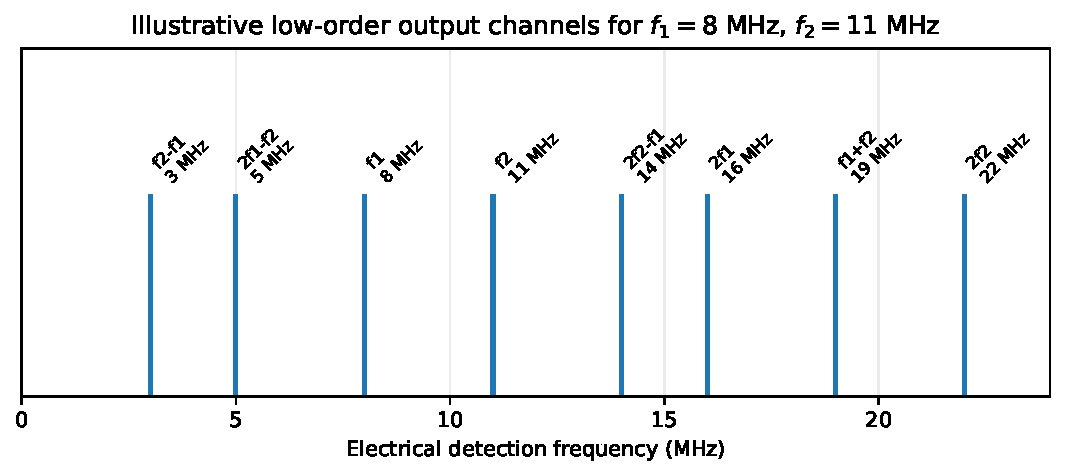
\includegraphics[width=0.83\linewidth]{../figures/fig2_rf_channel_map.pdf}
\caption{Illustrative frequency planning for $f_1=8$ MHz and $f_2=11$ MHz. Actual frequencies should be chosen after measuring raw-path bandwidth, spur locations, and MTS response.}
\end{figure}

\subsection{Non-atomic IM backgrounds}
The observed channel can contain
\begin{equation}
Z_{p,q}^{\rm meas}=Z_{p,q}^{\rm atom}+Z_{p,q}^{\rm EOM}+Z_{p,q}^{\rm RF}+Z_{p,q}^{\rm PD}+Z_{p,q}^{\rm ADC}+n_{p,q}.
\end{equation}
The first decisive experimental question is therefore not whether a spectral line exists, but whether the \emph{resonance-dependent increment} has the atomic scaling and phase expected for modulation transfer.

\section{The Synthetic Discriminator as an Optimal Estimator}

\subsection{Stacked real measurement vector}
Collect the selected quadratures into a real vector
\begin{equation}
\vect y(\nu)=
[I_{1,0},Q_{1,0},I_{0,1},Q_{0,1},I_{2,-1},Q_{2,-1},I_{-1,2},Q_{-1,2},\ldots]^T.
\end{equation}
Near the desired zero crossing,
\begin{equation}
\vect y\approx\vect y_0+\vect d_\nu\,\delta\nu+\vect n,
\qquad
\vect d_\nu=\left.\frac{\partial\vect y}{\partial\nu}\right|_{\nu_0}.
\end{equation}
Let the local channel-noise covariance be
\begin{equation}
\vect\Sigma=\mathrm E[\vect n\vect n^T].
\end{equation}
The off-diagonal terms matter: DDS spurs, laser intensity noise, photodetector noise, and common optical noise can correlate channels.

\subsection{Minimum-variance unbiased linear estimator}
Choose
\begin{equation}
\widehat{\delta\nu}=\vect w^T(\vect y-\vect y_0)
\end{equation}
with unbiasedness constraint
\begin{equation}
\vect w^T\vect d_\nu=1.
\end{equation}
Minimizing variance $\vect w^T\vect\Sigma\vect w$ gives
\begin{equation}
\boxed{
\vect w_{\rm opt}=
\frac{\vect\Sigma^{-1}\vect d_\nu}
{\vect d_\nu^T\vect\Sigma^{-1}\vect d_\nu}.}
\end{equation}
The corresponding variance is
\begin{equation}
\boxed{
\mathrm{Var}(\widehat{\delta\nu})=
\frac{1}{\vect d_\nu^T\vect\Sigma^{-1}\vect d_\nu}.}
\end{equation}
For local Gaussian statistics with parameter-independent covariance, the denominator is also the Fisher information carried by the selected measurement vector:
\begin{equation}
\boxed{\mathcal I_\nu=\vect d_\nu^T\vect\Sigma^{-1}\vect d_\nu.}
\end{equation}

\subsection{Interpretation}
The solution is a noise-whitened matched filter. It automatically gives more weight to channels that have large frequency derivative and less weight to channels that are noisy or redundant. In the special case of independent channels,
\begin{equation}
\mathcal I_\nu=\sum_k\frac{D_k^2}{\sigma_k^2}.
\end{equation}
Therefore no IM channel needs to outperform conventional MTS by itself. Several modest but independent channels can jointly improve the frequency estimate.

\begin{figure}[H]
\centering
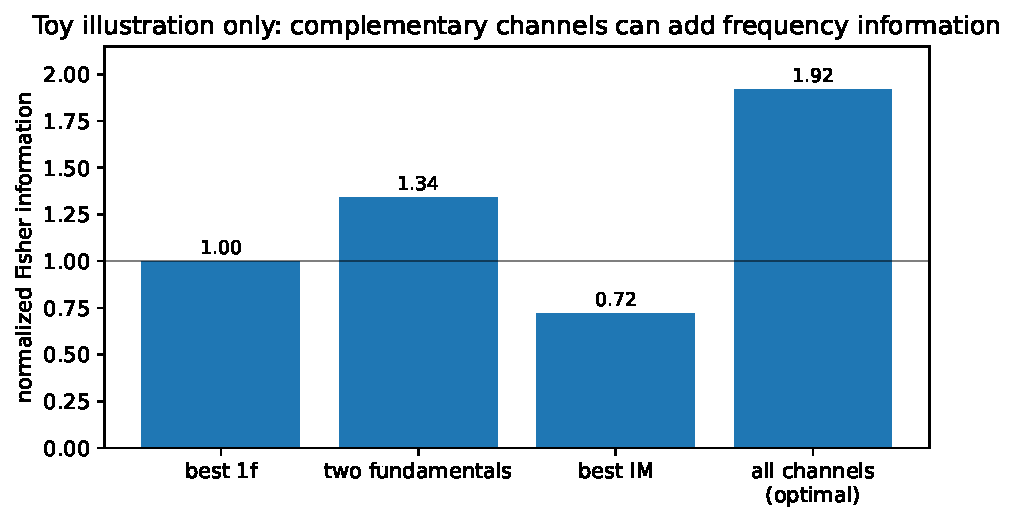
\includegraphics[width=0.70\linewidth]{../figures/fig4_information_toy.pdf}
\caption{Toy illustration only. The actual experiment must measure the covariance and slopes. The key hypothesis is that the nonlinear output channels contain complementary rather than fully redundant frequency information.}
\end{figure}

\subsection{Relation to the raw photocurrent information}
S-IMTS does not manufacture information. Let $i(t;\nu)$ denote the full raw photocurrent over an observation window. It contains some total information $\mathcal I_\nu^{\rm raw}$. Conventional single-channel MTS extracts a projection with information $\mathcal I_\nu^{1f}$; an S-IMTS channel bank extracts $\mathcal I_\nu^{\rm selected}$. A deep result would be
\begin{equation}
\mathcal I_\nu^{\rm selected}>\mathcal I_\nu^{1f}
\end{equation}
while still remaining below the raw-waveform bound. The paper can thus ask how much useful frequency information conventional demodulation discards.

\section{Constrained Synthetic Discriminators: Engineer a Property, Not Just Slope}

\subsection{First-order nuisance rejection}
Suppose the measurement responds to frequency, RAM amplitude $r$, optical power $P$, and demodulation-chain phase $\varphi$:
\begin{equation}
\delta\vect y=\vect d_\nu\delta\nu+\vect d_r\delta r+\vect d_P\delta P+\vect d_\varphi\delta\varphi+\vect n.
\end{equation}
Define
\begin{equation}
\vect A=[\vect d_\nu\ \vect d_r\ \vect d_P\ \vect d_\varphi],\qquad
\vect c=[1\ 0\ 0\ 0]^T.
\end{equation}
The minimum-noise weights satisfying $\vect A^T\vect w=\vect c$ are
\begin{equation}
\boxed{
\vect w=\vect\Sigma^{-1}\vect A
(\vect A^T\vect\Sigma^{-1}\vect A)^{-1}\vect c.}
\end{equation}
This creates a frequency estimator that is, to first order, blind to the calibrated nuisance directions while using the remaining channel dimensions to minimize noise.

\warningbox{Nuisance rejection is only possible if the frequency direction is not contained in the nuisance subspace. The condition number / principal angles of the whitened Jacobian must be reported. If a nuisance is experimentally indistinguishable from frequency, the correct result is ``not identifiable,'' not an aggressive correction.}

\subsection{Discriminator-shape synthesis}
The extra channels may also have different global detuning shapes. Sample them over a detuning grid $\{\Delta_j\}$ and choose a desired target error signal $e_{\rm tar}(\Delta)$. A regularized fit is
\begin{equation}
\boxed{
\min_{\vect w}
\sum_j\left[\vect w^T\vect y(\Delta_j)-e_{\rm tar}(\Delta_j)\right]^2
+\lambda\vect w^T\vect\Sigma\vect w.}
\end{equation}
A useful target is
\begin{equation}
e_{\rm tar}(\Delta)=A\tanh(\Delta/\Delta_0),
\end{equation}
which is linear near zero but bounded and monotonic over a broad region.

Additional constraints can be imposed at sampled points:
\begin{align}
e_{\rm syn}(0)&=0,\\
\left.\frac{\dd e_{\rm syn}}{\dd\Delta}\right|_0&\ge D_{\min},\\
e_{\rm syn}(\Delta_{j+1})-e_{\rm syn}(\Delta_j)&\ge 0\quad\text{for }\Delta_j>0,
\end{align}
with sign-reversed monotonicity for negative detuning. This converts the design into a quadratic program.

\begin{figure}[H]
\centering
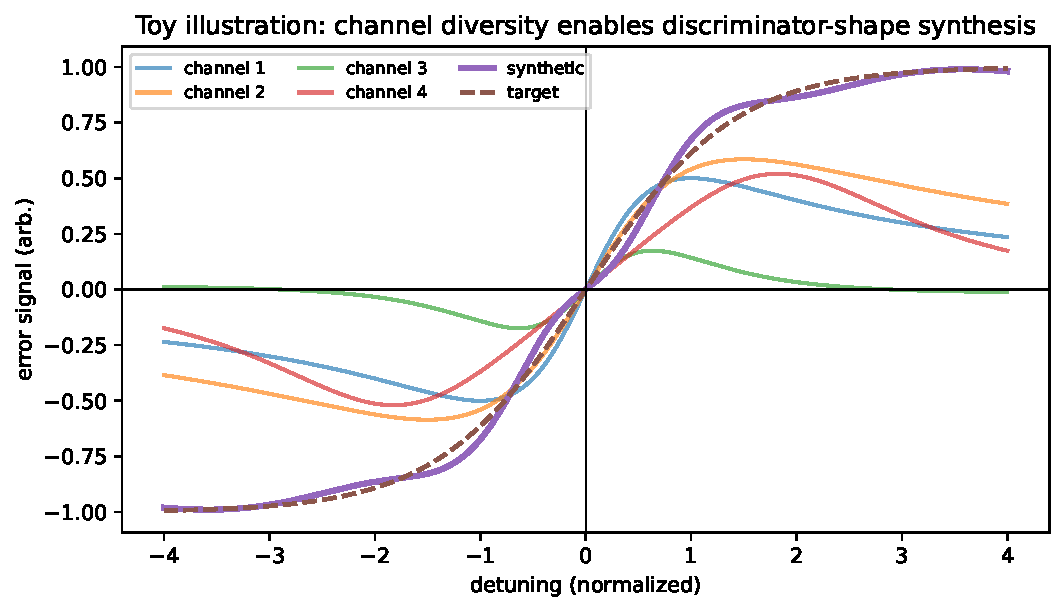
\includegraphics[width=0.82\linewidth]{../figures/fig3_shape_synthesis.pdf}
\caption{Toy basis-function example. Real MTS/IMTS line shapes must be measured. The purpose is to show the design principle: channel diversity can be used to approximate a desired global discriminator while penalizing noise.}
\end{figure}

\subsection{Feature suppression}
If undesired crossover or neighboring features appear differently across channels, define sampled vectors $\vect y_u$ at unwanted features and constrain
\begin{equation}
\vect w^T\vect y_u\approx0
\end{equation}
while maintaining large desired-transition derivative. This is a spectroscopy analogue of spatial null steering: the channels are not antennas, but the algebra of combining distinct complex observables is the same.

\section{Tunable IF and RF Frequency Planning}

\subsection{Center/difference parameterization}
Write the modulation tones as
\begin{equation}
\Omega_1=\Omega_c-\frac{\Omega_d}{2},\qquad
\Omega_2=\Omega_c+\frac{\Omega_d}{2}.
\end{equation}
Then
\begin{equation}
\Omega_2-\Omega_1=\Omega_d.
\end{equation}
This separates, to some extent, the scale of the optical sideband spacing around $\Omega_c$ from the electrical location of the difference-frequency readout $\Omega_d$. Classic two-tone FM spectroscopy already exploits analogous high-frequency excitation / convenient beat-frequency detection, so this is not standalone novelty. In S-IMTS it becomes one frequency-planning degree of freedom inside a larger multichannel atomic readout.

\subsection{Symmetric IM3 pair}
The third-order pair is
\begin{align}
2\Omega_1-\Omega_2&=\Omega_c-\frac{3\Omega_d}{2},\\
2\Omega_2-\Omega_1&=\Omega_c+\frac{3\Omega_d}{2}.
\end{align}
These channels move symmetrically around $\Omega_c$ as the tone spacing changes. They are attractive because a purely linear electrical transfer of the two input tones cannot generate those electrical frequencies, although EOM and detector nonlinearities can. Their paired complex responses may also provide useful symmetry checks.

\subsection{Noise-aware frequency planning}
Let the measured electronics/photodetector voltage-noise PSD be $S_V(f)$. A simple design problem is
\begin{equation}
\min_{\Omega_1,\Omega_2,(p,q)}
\frac{S_V(|p\Omega_1+q\Omega_2|)}{|D_{p,q}|^2}
\end{equation}
subject to the atomic response and hardware bandwidth constraints. The attractive instrumentation question is whether useful atomic information can be placed in a quiet RF region rather than accepting the noise/spur environment of one fixed modulation frequency.

\section{Dynamic Discriminator and Closed-Loop Consequences}

\subsection{Static slope is not enough}
For small laser-frequency modulation at servo Fourier frequency $\omega$ around a fixed lock point, each channel has a dynamic discriminator
\begin{equation}
D_k(\ii\omega)=\frac{\delta e_k(\ii\omega)}{\delta\nu(\ii\omega)}.
\end{equation}
For fixed weights,
\begin{equation}
D_{\rm syn}(\ii\omega)=\vect w^T\vect D(\ii\omega).
\end{equation}
If $A(\ii\omega)$ is the current-to-frequency actuator and $C(\ii\omega)$ the controller,
\begin{equation}
L(\ii\omega)=C(\ii\omega)A(\ii\omega)D_{\rm syn}(\ii\omega).
\end{equation}
Thus an IM channel with a smaller DC slope could still be attractive if its dynamic phase is more favorable at high feedback frequencies. Conversely, a large DC slope does not prove high usable loop bandwidth.

\subsection{Static vs frequency-dependent combining weights}
The first paper should use static channel weights: they are easy to calibrate and keep latency low. A more general multichannel Wiener solution can use frequency-dependent weights
\begin{equation}
\vect w(\omega)\propto\vect S_n^{-1}(\omega)\vect d_\nu(\omega),
\end{equation}
which effectively makes a MIMO digital filter bank. This is powerful but changes the servo phase and is better treated as future work after the static synthetic-discriminator concept is validated.

\subsection{Latency architecture for POSM}
The current hybrid lock should be preserved during discovery:
\begin{enumerate}
\item Keep analog-demodulated ADC\_CH0 and the short PI loop as the stable reference implementation.
\item Use raw ADC\_CH1 for simultaneous complex demodulation of multiple output frequencies during scans and locked operation.
\item Compute the first optimal weights on the host from captured channel slopes and covariance.
\item Only after performance is demonstrated offline, move a small selected digital demod bank and weighted sum into FPGA logic.
\item Re-measure total latency and dynamic discriminator before attempting a MHz-class synthetic-error fast loop.
\end{enumerate}

\section{Experimental Program: Fast Go/No-Go Before a Full Paper}

\subsection{Stage 0 - electrical and optical IMD baseline}
Before placing scientific meaning on any IM channel, measure the entire RF chain with the laser far from resonance and with appropriate optical blocks. For every candidate $f_{p,q}$ record amplitude and phase versus RF drive power. Useful configurations are:
\begin{enumerate}
\item two-tone RF source into the EOM chain with no atomic resonance contribution;
\item laser far detuned from the selected Rb line;
\item pump blocked;
\item pump/probe spatial overlap deliberately removed;
\item cell temperature / Rb density varied if practical.
\end{enumerate}
The atomically resonant increment should track the spectroscopy condition rather than a static RF spur.

\subsection{Stage 1 - two-tone spectral map}
Choose two nondegenerate tones within the verified EOM, photodetector and ADC bandwidths. One illustrative pair is 8 and 11 MHz, but the final choice should follow measured hardware response and conventional MTS optimization. During a slow laser scan, digitally record complex amplitudes at low-order channels such as
\begin{equation}
\{f_2-f_1,\ 2f_1-f_2,\ f_1,\ f_2,\ 2f_2-f_1,\ f_1+f_2,\ 2f_1,\ 2f_2\}.
\end{equation}
For each channel map $I(\Delta)$, $Q(\Delta)$, amplitude, phase, zero-crossing slope, and baseline.

\subsection{Stage 2 - atomic-origin tests}
A candidate channel should pass several of the following:
\begin{itemize}
\item resonance dependence disappears far from Rb;
\item pump blocking removes modulation transfer;
\item beam-overlap degradation reduces the resonant component;
\item channel phase changes with the expected integer combination of input phases;
\item modulation-index scaling is consistent with a low-order pathway over a controlled small-signal region;
\item dependence on pump/probe power and polarization is physically consistent and reproducible.
\end{itemize}
No one test alone proves microscopic FWM origin; the combination establishes a credible atomic attribution.

\subsection{Stage 3 - information audit}
At the target zero crossing, measure
\begin{equation}
\vect d_\nu
\end{equation}
using a calibrated small frequency dither or slow calibrated scan, and measure
\begin{equation}
\vect\Sigma(f)
\end{equation}
from locked or stationary data. Compare four cases:
\begin{enumerate}
\item best conventional single-tone MTS channel;
\item the two fundamental channels only;
\item best individual true IM channel;
\item all selected fundamental + IM channels with optimal weights.
\end{enumerate}
The decisive local result is an equivalent frequency-noise reduction or measured Fisher-information increase that survives equal-resource normalization.

\subsection{Stage 4 - one engineered property}
Do not attempt to optimize every imaginable property in paper 1. Choose one secondary result:
\begin{itemize}
\item \textbf{wide-range discriminator:} steep center plus larger monotonic capture range;
\item \textbf{RAM-insensitive discriminator:} first-order null to measured RAM perturbation;
\item \textbf{RF-noise avoidance:} move/weight channels around measured RF spurs;
\item \textbf{feature suppression:} cancel a specific unwanted crossover/background component.
\end{itemize}
The strongest general-purpose combination is likely minimum equivalent frequency noise as the primary metric and broad monotonic capture as the secondary metric.

\subsection{Stage 5 - close the loop}
Compare actual locks under equal total optical power and equal total modulation-drive budget. Report:
\begin{itemize}
\item equivalent in-loop frequency-noise PSD;
\item out-of-loop beat/discriminator noise when available;
\item unity-gain frequency and phase margin;
\item servo bump / sensitivity peak;
\item capture/recovery range;
\item Allan deviation or long-duration frequency stability if the experiment duration permits;
\item sensitivity to RAM/power if claimed.
\end{itemize}

\section{Fair Comparison and Resource Accounting}

A synthetic or multi-frequency method can appear better simply because it uses more optical sidebands, more RF power, or more detector bandwidth. The comparison should freeze or explicitly report:
\begin{itemize}
\item total pump optical power incident on the cell;
\item probe optical power and beam sizes;
\item total RF power delivered to the EOM or a physically justified modulation-index budget;
\item detector gain/bandwidth and ADC scaling;
\item same atomic transition, cell temperature, polarization and alignment;
\item same observation time / equivalent noise bandwidth;
\item same laser actuator/controller when comparing locked performance.
\end{itemize}
Velocity-comb MTS is especially important here: it already demonstrates that additional optical frequency components can improve stability by engaging more velocity classes. S-IMTS must show that its improvement is tied to output-channel diversity / optimal measurement rather than merely extra optical power or extra atoms.

\section{Novelty Map: What the Paper Is and Is Not}

\begin{tabularx}{\linewidth}{>{\raggedright\arraybackslash}p{0.24\linewidth}X X}
\toprule
\textbf{Prior concept} & \textbf{What is already established} & \textbf{Proposed S-IMTS distinction}\\
\midrule
Single-tone optimized MTS & Tune modulation frequency/index, phase, power, beam size for strong slope/amplitude and good locking. & Treat the RF output as a multichannel object, including true combination-frequency channels.\\
\addlinespace
Two-tone FM spectroscopy & Two modulation frequencies and beat / convenient-IF detection are classic. & Doppler-free MTS nonlinear transfer plus true IM output channels and joint synthetic frequency estimator.\\
\addlinespace
Simultaneous / multi-frequency MTS & Different modulation frequencies can multiplex transitions/species. & Channels correspond to the same atomic lock and are jointly combined rather than merely separated.\\
\addlinespace
Velocity-comb MTS & Multiple optical frequencies engage different velocity groups and can improve stability. & Test information residing in multiple electrical output channels under equal resource conditions.\\
\addlinespace
Dual-frequency MTS patent CN122178176A & Demodulate at $f_1$ and $f_2$ and add two fundamental error signals to improve slope + amplitude. & Explicitly demodulate at $p f_1+q f_2$, characterize IM channel diversity, and compute optimal covariance-aware / constrained weights.\\
\addlinespace
Synthetic FM triplet & Programmable optical modulation can engineer a cleaner frequency discriminator / RAM behavior. & Synthetic response is assembled from the nonlinear atomic intermodulation output space rather than only from programmed input sidebands.\\
\bottomrule
\end{tabularx}

\vspace{0.15in}
\warningbox{Working novelty statement only: ``Two-tone MTS produces multiple resonant intermodulation channels containing complementary frequency information, and optimal coherent combination of those channels yields a synthetic atomic discriminator with properties unavailable from any individual MTS channel.'' This statement must be weakened or changed if the literature/patent search finds a direct predecessor or if the channels are experimentally redundant.}

\section{Failure Modes and What Each Failure Would Teach Us}

\begin{tabularx}{\linewidth}{>{\bfseries}p{0.28\linewidth}X}
All IM channels are dominated by RF/EOM spurs & The spectroscopy idea fails quickly; useful hardware result is an RF linearity budget. Do not force a paper.\\
Atomic IM channels exist but are extremely weak & Could still be a nonlinear-spectroscopy note if scaling/pathway physics is clean, but not a better lock.\\
IM channels are scalar copies of fundamentals & Fisher information gain is negligible; synthetic readout offers little beyond averaging.\\
IM channels differ but noises are fully correlated & Slopes alone look diverse but optimal covariance weighting shows little real sensitivity gain.\\
Noise-optimal combination helps but capture range worsens & Still publishable if the declared metric is local frequency noise; capture can remain handled by legacy acquisition.\\
Shape engineering works but adds digital latency & Use the synthetic channel as a slow/global observer and preserve analog fast feedback, or implement a small FPGA demod bank.\\
A nuisance direction is collinear with frequency & It cannot be rejected without sacrificing frequency information; report the conditioning honestly.\\
Microscopic model disagrees & Do not overfit $\chi^{(3)}$. Use density-matrix / neighboring-transition / spontaneous-emission mechanisms as needed.\\
\end{tabularx}

\section{Recommended Paper Focus}

The cleanest first paper should avoid becoming a catalog of every possible knob. A disciplined hierarchy is:

\subsection*{Primary result - frequency-information enhancement}
Demonstrate that the joint channel vector has
\begin{equation}
\mathcal I_\nu^{\rm S-IMTS}>\mathcal I_\nu^{\rm best\ conventional}
\end{equation}
under equal optical/RF budgets, and show a corresponding measured reduction of equivalent frequency noise.

\subsection*{Secondary result - engineered global discriminator}
Use the same channel set to synthesize a broad monotonic error signal while preserving a declared center slope/noise penalty. This gives a visually and operationally intuitive advantage beyond a local information metric.

\subsection*{Tertiary result - actual locking}
Close a laser lock using the synthetic discriminator and compare conventional single-tone, dual-fundamental, best individual IM, and synthetic IMTS. Out-of-loop validation materially strengthens the claim.

A suitable title is:
\begin{center}
\textbf{Synthetic Intermodulation Transfer Spectroscopy for Engineered Atomic Frequency Discrimination}
\end{center}

A conservative abstract-level claim would be:

\begin{quote}
We introduce a two-tone modulation-transfer spectroscopy protocol in which the complex fundamental and combination-frequency components of the probe photocurrent are treated as a multichannel measurement of laser detuning. We map resonant intermodulation channels in rubidium, quantify their channel-to-channel noise covariance and frequency response, and synthesize a minimum-noise atomic discriminator from the measured channel vector. We further demonstrate constrained line-shape synthesis as an example of engineering a discriminator property beyond conventional single-frequency MTS.
\end{quote}

\section{POSM-Specific Implementation Plan}

\begin{tabularx}{\linewidth}{p{0.11\linewidth}p{0.25\linewidth}X}
\toprule
\textbf{Phase} & \textbf{Goal} & \textbf{Exit criterion}\\
\midrule
0 & Freeze baseline and measure RF linearity & Two-tone source/EOM/PD/ADC spur map exists with laser far detuned.\\
1 & Add two-tone pump + offline demod bank & Complex traces for fundamentals, difference, sum and IM3 pair are captured during an Rb scan.\\
2 & Establish atomic IM channels & At least one non-fundamental channel passes resonance, pump-block, overlap, scaling and phase checks.\\
3 & Information audit & $\vect d_\nu$, $\vect\Sigma$ and optimal weights are measured; comparison to best 1f baseline is statistically repeatable.\\
4 & Synthetic property & One constrained discriminator (noise-optimal or broad-monotonic) shows a measurable advantage.\\
5 & Closed-loop test & Synthetic channel drives a stable lock; bandwidth/noise/capture are compared fairly to conventional MTS.\\
\bottomrule
\end{tabularx}

\subsection{Hardware modifications kept minimal}
The current AD9959 allocation already provides multiple coherent DDS channels. A practical prototype can use one channel for $f_1$ and a spare/reserved channel for $f_2$, combine them with an RF power combiner, and retain the conventional mixer LO channel for baseline operation. Exact amplitudes must be calibrated at the EOM because cable, combiner and amplifier gains differ with frequency. The raw RF ADC path is the key measurement path; analog bandwidth and Nyquist constraints must be measured before choosing the highest output channel.

\subsection{FPGA/host partitioning}
First implementation:
\begin{itemize}
\item FPGA: capture raw RF blocks with coherent timestamps / known sample clock.
\item Host: numerically demodulate selected $p,q$ channels, calibrate phase, fit line shapes, estimate covariance and solve for weights.
\item FPGA later: implement a bank of complex mixers/NCOs, CIC/FIR decimation and a weighted accumulator only after the channel set is fixed.
\end{itemize}
This keeps the research agile and prevents premature gateware optimization.

\section{Paper-Ready Figures and Tables to Produce}

A strong 4--6 page eventual article could be built around five figures:
\begin{enumerate}
\item \textbf{Concept figure:} two-tone pump, 2D optical sideband lattice, atomic medium, output RF channel bank.
\item \textbf{IM spectrum map:} color map of $|Z_{p,q}(\Delta)|$ or selected complex line shapes with controls showing atomic origin.
\item \textbf{Information figure:} $D_k$, channel covariance, per-channel information and cumulative/optimal information.
\item \textbf{Synthetic discriminator figure:} conventional 1f, dual-fundamental, best IM, and optimized synthetic line shape/noise.
\item \textbf{Lock figure:} frequency-noise PSD / transfer function / Allan deviation or capture result for conventional vs S-IMTS.
\end{enumerate}

Tables should include equal-resource settings, modulation frequencies/indices, optical powers, detector bandwidths, channel list, and uncertainty/repeatability.

\section{Selected Literature Reading Map}

The bundled \texttt{literature/READING\_LIST.md} gives a larger map. The most important papers to read in order are:
\begin{enumerate}
\item Shirley (1982) and Camy/Borde/Ducloy (1982): origin of modulation transfer.
\item McCarron/King/Cornish (2008): Rb MTS and practical FWM picture.
\item Noh et al. (2011) and Innes et al. (2024): density-matrix MTS theory.
\item Preuschoff/Schlosser/Birkl (2018/2020): conventional modulation-parameter optimization baseline.
\item Janik/Carlisle/Gallagher (1986): two-tone FM prior art; critical for tunable-IF novelty boundary.
\item Schine/Ranjit/Majumder (2013): high-depth multi-harmonic FM detection formalism.
\item Mihm et al. (2018), Guan et al. (2025), Miao et al. (2025): multi-frequency / multi-output MTS neighbors.
\item CN122178176A (2026): closest dual-frequency MTS patent; two fundamental demodulations are added for slope/amplitude improvement.
\item Kedar et al. (2024) and Eguchi et al. (2026): synthetic modulation as an engineered discriminator concept.
\item Khan et al. (2025): reminder that real MTS can involve neighboring transitions and spontaneous-emission-mediated contributions.
\end{enumerate}

\section{References}
\small
\begin{enumerate}[label={[\arabic*]},leftmargin=2.0em]
\item J. H. Shirley, ``Modulation transfer processes in optical heterodyne saturation spectroscopy,'' \emph{Opt. Lett.} 7, 537--539 (1982). \url{https://doi.org/10.1364/OL.7.000537}
\item G. Camy, Ch. J. Bord\'e, M. Ducloy, ``Heterodyne saturation spectroscopy through frequency modulation of the saturating beam,'' \emph{Opt. Commun.} 41, 325--330 (1982). \url{https://doi.org/10.1016/0030-4018(82)90406-0}
\item D. J. McCarron, S. A. King, S. L. Cornish, ``Modulation transfer spectroscopy in atomic rubidium,'' \emph{Meas. Sci. Technol.} 19, 105601 (2008). \url{https://arxiv.org/abs/0805.2708}
\item H.-R. Noh et al., ``Modulation transfer spectroscopy for 87Rb atoms: theory and experiment,'' \emph{Opt. Express} 19, 23444 (2011). \url{https://doi.org/10.1364/OE.19.023444}
\item T. Preuschoff, M. Schlosser, G. Birkl, ``Optimization strategies for modulation transfer spectroscopy applied to laser stabilization,'' \emph{Opt. Express} 26, 24010 (2018). \url{https://arxiv.org/abs/2003.12035}
\item A. D. Innes, P. Majumder, H.-R. Noh, S. L. Cornish, ``Modulation Transfer Spectroscopy of the D1 Transition of Potassium: Theory and Experiment,'' \emph{J. Phys. B} 57, 075401 (2024). \url{https://arxiv.org/abs/2310.11327}
\item S. Khan, H.-R. Noh, J.-T. Kim, ``Neighboring and polarization effects on line shape of the modulation transfer spectroscopy in lower ground hyperfine state of Rb atoms,'' \emph{Sci. Rep.} 15, 7713 (2025). \url{https://doi.org/10.1038/s41598-025-92562-z}
\item G. R. Janik, C. B. Carlisle, T. F. Gallagher, ``Two-tone frequency-modulation spectroscopy,'' \emph{JOSA B} 3, 1070--1074 (1986). \url{https://doi.org/10.1364/JOSAB.3.001070}
\item V. Avetisov, M. Kauranen, ``Two-tone frequency-modulation spectroscopy for quantitative measurements of gaseous species,'' \emph{Appl. Opt.} 35, 4705--4723 (1996). \url{https://doi.org/10.1364/AO.35.004705}
\item E. A. Whittaker et al., ``Reduction of residual amplitude modulation in frequency-modulation spectroscopy by using harmonic frequency modulation,'' \emph{JOSA B} 5, 1253 (1988). \url{https://doi.org/10.1364/JOSAB.5.001253}
\item R. Schine, G. Ranjit, P. K. Majumder, ``Frequency Modulation Spectroscopy at High Modulation Depth in an Indium Atomic Beam,'' arXiv:1310.6465 (2013). \url{https://arxiv.org/abs/1310.6465}
\item M. Mihm et al., ``Simultaneous modulation transfer spectroscopy on transitions of multiple atomic species for compact laser frequency reference modules,'' \emph{Rev. Sci. Instrum.} 89, 096101 (2018). \url{https://arxiv.org/abs/1806.02606}
\item A. Perez Galvan et al., ``Two-color modulation transfer spectroscopy,'' arXiv:0812.1386 (2008). \url{https://arxiv.org/abs/0812.1386}
\item X. Guan et al., ``Velocity-comb modulation transfer spectroscopy,'' arXiv:2501.16148 / \emph{Phys. Rev. Applied} (2025). \url{https://arxiv.org/abs/2501.16148}
\item J. Miao et al., ``Single-Atomic-Ensemble Dual-Wavelength Optical Standard,'' arXiv:2411.02107 / \emph{Photonics Research} (2025). \url{https://arxiv.org/abs/2411.02107}
\item D. Kedar et al., ``Synthetic FM triplet for AM-free precision laser stabilization and spectroscopy,'' \emph{Optica} 11, 58--63 (2024). \url{https://arxiv.org/abs/2311.14268}
\item K. Eguchi et al., ``Terahertz Synthetic FM Triplet for Distortion-Free Stabilization and Lamb-Dip Spectroscopy,'' arXiv:2602.07737 (2026). \url{https://arxiv.org/abs/2602.07737}
\item R. J. Thomas et al., ``Optimal strategies for low-noise detection of atoms using resonant frequency modulation spectroscopy in cold atom interferometers,'' arXiv:2408.06575 (2024). \url{https://arxiv.org/abs/2408.06575}
\item V. Negnevitsky, L. D. Turner, ``Wideband laser locking to an atomic reference with modulation transfer spectroscopy,'' \emph{Opt. Express} 21, 3103--3113 (2013). \url{https://doi.org/10.1364/OE.21.003103}
\item S. Lee et al., ``Laser frequency stabilization in the 10$^{-14}$ range via optimized modulation transfer spectroscopy on the 87Rb D2 line,'' \emph{Opt. Lett.} 48, 1020--1023 (2023). \url{https://opg.optica.org/ol/abstract.cfm?uri=ol-48-4-1020}
\item CN122178176A, ``Dual-frequency modulation transfer spectroscopy laser frequency stabilization device and method,'' Zhejiang Sci-Tech University, published 9 June 2026. \url{https://eureka.patsnap.com/patent-CN122178176A}
\item POSM, ``FPGA MTS Laser-Lock Core Onboarding Packet v3 Draft,'' internal project packet (2026).
\item POSM, ``Polarization Tap and Stokes Polarimeter Onboarding Packet v1 Draft,'' internal project packet (2026).
\end{enumerate}

\normalsize
\section*{Final Research Position}
S-IMTS is worth testing because it has an unusually favorable risk structure. The first falsification experiment is cheap: two coherent tones, raw RF capture, digital demodulation and careful controls. If the output combination-frequency channels are weak, non-atomic, or redundant, the project can be stopped quickly. If they are atomically resonant and carry complementary information, the same data immediately supports a rigorous matched-filter / Fisher-information analysis and a synthetic-discriminator demonstration. The highest-value result is not ``a new peak'' or ``more slope''; it is evidence that conventional MTS leaves exploitable frequency information in a nonlinear RF output space and that engineered readout of this space produces a measurably better atomic frequency sensor.

\end{document}
